\documentclass{standalone}

\usepackage{comment}
\usepackage{siunitx}
\usepackage{tikz}

\DeclareSIUnit \parsec {pc}
\DeclareSIUnit \ly {ly}

\usetikzlibrary{shapes.geometric}
\usetikzlibrary{decorations,calligraphy}

\begin{document}

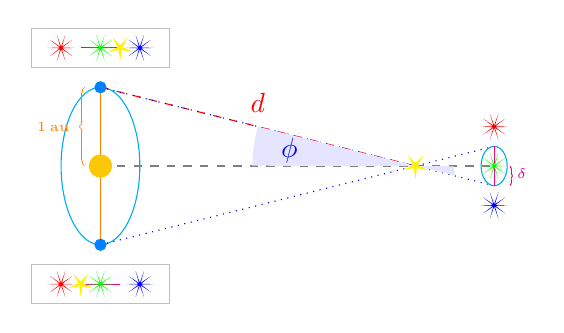
\begin{tikzpicture}
    \node[ellipse,
    draw=cyan,
    minimum width=1cm,
    minimum height=2cm] (e1) at (0,0) {};
    
\draw[dashed, color=red] (0,1) node[xshift=2cm, yshift=-0.2cm]{$\textcolor{red}{d}$} -- (4,0);
    
    \draw[dotted, color=blue] (0,1) -- (5,-0.25);
    \draw[dotted, color=blue] (0,-1) -- (5,0.25);
    
    \draw[dashed, color=gray] (0,0) -- (4,0);
    \draw[color=orange] (0,1) -- (0,-1);
    
    \draw[color=orange, pen colour=orange, decorate, decoration={calligraphic brace, amplitude=2pt}] (-0.2,0) node[xshift=-0.4cm, yshift=0.5cm]{\tiny $\SI{1}{\astronomicalunit}$} -- (-0.2,1);
    
    \fill[color=white!90!blue] (4,0)  -- (2,0.5) arc (164:180:1.8);
    \node at (2.4,0.2){$\textcolor{blue}{\phi}$};
    
    \node[ellipse,
    draw=cyan,
    minimum width=0.25cm,
    minimum height=0.5cm] (e2) at (5,0) {};
    
    \draw[dashed, color=gray] (4,0) -- (5,0);
    \draw[color=magenta] (5, 0.25) -- (5,-0.25);
    \draw[color=magenta, pen colour=magenta, decorate, decoration={calligraphic brace, amplitude=1pt}] (5.2, 0.0) node[xshift=0.15cm, yshift=-0.1cm]{\tiny $\textcolor{magenta}{\delta}$} -- (5.2,-0.25);
    
    1\fill[color=white!90!blue] (4,0) -- (4.5,-0.12) arc (0:13.5:0.5);
    
    \node[star, star points=5, star point ratio=0.2, fill=yellow] (s0) at (4,0) {};
    
    \node[star, star points=10, star point ratio=0.1, fill=red] (s1) at (5, 0.5) {};
    \node[star, star points=10, star point ratio=0.1, fill=green] (s2) at (5, 0) {};
    \node[star, star points=10, star point ratio=0.1, fill=blue] (s3) at (5, -0.5) {};
    
       
    \node[rectangle,
    draw=lightgray,
    minimum width=1.75cm,
    minimum height=0.5cm] (r1) at (0,1.5) {};    

    \draw[color=magenta] (-0.25, 1.5) -- (0.25, 1.5);
    \node[star, star points=10, star point ratio=0.1, fill=red] (r1s1) at (-0.5, 1.5) {};
    \node[star, star points=10, star point ratio=0.1, fill=green] (r1s2) at (0, 1.5) {};
    \node[star, star points=5, star point ratio=0.2, fill=yellow] (r1s0) at (0.25, 1.5) {};
    \node[star, star points=10, star point ratio=0.1, fill=blue] (r1s3) at (0.5, 1.5) {};
    

    \node[rectangle,
    draw=lightgray,
    minimum width=1.75cm,
    minimum height=0.5cm] (r1) at (0,-1.5) {};
    
    \draw[color=magenta] (-0.25, -1.5) -- (0.25, -1.5);
    \node[star, star points=10, star point ratio=0.1, fill=red] (r1s1) at (-0.5, -1.5) {};
    \node[star, star points=5, star point ratio=0.2, fill=yellow] (r1s0) at (-0.25, -1.5) {};
    \node[star, star points=10, star point ratio=0.1, fill=green] (r1s2) at (0, -1.5) {};
    \node[star, star points=10, star point ratio=0.1, fill=blue] (r1s3) at (0.5, -1.5) {};

    \draw[fill, color=yellow!60!orange] (0,0) circle[radius=4pt];
    \draw[fill, color=blue!50!cyan] (0,1) circle[radius=2pt];
    \draw[fill, color=blue!50!cyan] (0,-1) circle[radius=2pt];
    
\end{tikzpicture}

\end{document}
